\documentclass{article}
\usepackage[margin=1in]{geometry}
\usepackage[linesnumbered,ruled,vlined]{algorithm2e}
\usepackage{amsfonts}
\usepackage{amsmath}
\usepackage{amssymb}
\usepackage{amsthm}
\usepackage{enumitem}
\usepackage{fancyhdr}
\usepackage{hyperref}
\usepackage{minted}
\usepackage{multicol}
\usepackage{pdfpages}
\usepackage{standalone}
\usepackage[many]{tcolorbox}
\usepackage{tikz-cd}
\usepackage{transparent}
\usepackage{xcolor}
% \tcbuselibrary{minted}

\author{Nathan Solomon}

\newcommand{\fig}[1]{
    \begin{center}
        \includegraphics[width=\textwidth]{#1}
    \end{center}
}

% Math commands
\renewcommand{\d}{\mathrm{d}}
\DeclareMathOperator{\id}{id}
\DeclareMathOperator{\im}{im}
\DeclareMathOperator{\proj}{proj}
\DeclareMathOperator{\Span}{span}
\DeclareMathOperator{\Tr}{Tr}
\DeclareMathOperator{\tr}{tr}
\DeclareMathOperator{\ad}{ad}
\DeclareMathOperator{\ord}{ord}
%%%%%%%%%%%%%%% \DeclareMathOperator{\sgn}{sgn}
\DeclareMathOperator{\Aut}{Aut}
\DeclareMathOperator{\Inn}{Inn}
\DeclareMathOperator{\Out}{Out}
\DeclareMathOperator{\stab}{stab}

\newcommand{\N}{\ensuremath{\mathbb{N}}}
\newcommand{\Z}{\ensuremath{\mathbb{Z}}}
\newcommand{\Q}{\ensuremath{\mathbb{Q}}}
\newcommand{\R}{\ensuremath{\mathbb{R}}}
\newcommand{\C}{\ensuremath{\mathbb{C}}}
\renewcommand{\H}{\ensuremath{\mathbb{H}}}
\newcommand{\F}{\ensuremath{\mathbb{F}}}

\newcommand{\E}{\ensuremath{\mathbb{E}}}
\renewcommand{\P}{\ensuremath{\mathbb{P}}}

\newcommand{\es}{\ensuremath{\varnothing}}
\newcommand{\inv}{\ensuremath{^{-1}}}
\newcommand{\eps}{\ensuremath{\varepsilon}}
\newcommand{\del}{\ensuremath{\partial}}
\renewcommand{\a}{\ensuremath{\alpha}}

\newcommand{\abs}[1]{\ensuremath{\left\lvert #1 \right\rvert}}
\newcommand{\norm}[1]{\ensuremath{\left\lVert #1\right\rVert}}
\newcommand{\mean}[1]{\ensuremath{\left\langle #1 \right\rangle}}
\newcommand{\floor}[1]{\ensuremath{\left\lfloor #1 \right\rfloor}}
\newcommand{\ceil}[1]{\ensuremath{\left\lceil #1 \right\rceil}}
\newcommand{\bra}[1]{\ensuremath{\left\langle #1 \right\rvert}}
\newcommand{\ket}[1]{\ensuremath{\left\lvert #1 \right\rangle}}
\newcommand{\braket}[2]{\ensuremath{\left.\left\langle #1\right\vert #2 \right\rangle}}

\newcommand{\catname}[1]{{\normalfont\textbf{#1}}}

\newcommand{\up}{\ensuremath{\uparrow}}
\newcommand{\down}{\ensuremath{\downarrow}}

% Custom environments
\newtheorem{thm}{Theorem}[section]

\definecolor{probBackgroundColor}{RGB}{250,240,240}
\definecolor{probAccentColor}{RGB}{140,40,0}
\newenvironment{prob}{
    \stepcounter{thm}
    \begin{tcolorbox}[
        boxrule=1pt,
        sharp corners,
        colback=probBackgroundColor,
        colframe=probAccentColor,
        borderline west={4pt}{0pt}{probAccentColor},
        breakable
    ]
    \color{probAccentColor}\textbf{Problem \thethm.} \color{black}
} {
    \end{tcolorbox}
}

\definecolor{exampleBackgroundColor}{RGB}{212,232,246}
\newenvironment{example}{
    \stepcounter{thm}
    \begin{tcolorbox}[
      boxrule=1pt,
      sharp corners,
      colback=exampleBackgroundColor,
      breakable
    ]
    \textbf{Example \thethm.}
} {
    \end{tcolorbox}
}

\definecolor{propBackgroundColor}{RGB}{255,245,220}
\definecolor{propAccentColor}{RGB}{150,100,0}
\newenvironment{prop}{
    \stepcounter{thm}
    \begin{tcolorbox}[
        boxrule=1pt,
        sharp corners,
        colback=propBackgroundColor,
        colframe=propAccentColor,
        breakable
    ]
    \color{propAccentColor}\textbf{Proposition \thethm. }\color{black}
} {
    \end{tcolorbox}
}

\definecolor{thmBackgroundColor}{RGB}{235,225,245}
\definecolor{thmAccentColor}{RGB}{50,0,100}
\renewenvironment{thm}{
    \stepcounter{thm}
    \begin{tcolorbox}[
        boxrule=1pt,
        sharp corners,
        colback=thmBackgroundColor,
        colframe=thmAccentColor,
        breakable
    ]
    \color{thmAccentColor}\textbf{Theorem \thethm. }\color{black}
} {
    \end{tcolorbox}
}

\definecolor{corBackgroundColor}{RGB}{240,250,250}
\definecolor{corAccentColor}{RGB}{50,100,100}
\newenvironment{cor}{
    \stepcounter{thm}
    \begin{tcolorbox}[
        enhanced,
        boxrule=0pt,
        frame hidden,
        sharp corners,
        colback=corBackgroundColor,
        borderline west={4pt}{0pt}{corAccentColor},
        breakable
    ]
    \color{corAccentColor}\textbf{Corollary \thethm. }\color{black}
} {
    \end{tcolorbox}
}

\definecolor{lemBackgroundColor}{RGB}{255,245,235}
\definecolor{lemAccentColor}{RGB}{250,125,0}
\newenvironment{lem}{
    \stepcounter{thm}
    \begin{tcolorbox}[
        enhanced,
        boxrule=0pt,
        frame hidden,
        sharp corners,
        colback=lemBackgroundColor,
        borderline west={4pt}{0pt}{lemAccentColor},
        breakable
    ]
    \color{lemAccentColor}\textbf{Lemma \thethm. }\color{black}
} {
    \end{tcolorbox}
}

\definecolor{proofBackgroundColor}{RGB}{255,255,255}
\definecolor{proofAccentColor}{RGB}{80,80,80}
\renewenvironment{proof}{
    \begin{tcolorbox}[
        enhanced,
        boxrule=1pt,
        sharp corners,
        colback=proofBackgroundColor,
        colframe=proofAccentColor,
        borderline west={4pt}{0pt}{proofAccentColor},
        breakable
    ]
    \color{proofAccentColor}\emph{\textbf{Proof. }}\color{black}
} {
    \qed \end{tcolorbox}
}

\definecolor{noteBackgroundColor}{RGB}{240,250,240}
\definecolor{noteAccentColor}{RGB}{30,130,30}
\newenvironment{note}{
    \begin{tcolorbox}[
        enhanced,
        boxrule=0pt,
        frame hidden,
        sharp corners,
        colback=noteBackgroundColor,
        borderline west={4pt}{0pt}{noteAccentColor},
        breakable
    ]
    \color{noteAccentColor}\textbf{Note. }\color{black}
} {
    \end{tcolorbox}
}


\fancyhf{}
\setlength{\headheight}{24pt}

\date{\today}
\title{Physics 245 Homework \#8}

\begin{document}
\maketitle

\begin{prob}
\end{prob}
\begin{enumerate}[label=(\alph*)]
    \item
        \[ T = \begin{bmatrix}
            1 & 0 \\
            0 & e^{i\pi/4}
        \end{bmatrix} = e^{i\pi/8} \begin{bmatrix}
            e^{-i\pi/8} & 0 \\
            0 & e^{i\pi/8}
        \end{bmatrix} = e^{i\pi/8} R_z(\pi/4). \]
    \item \begin{align*}
            HTH &= \left( \frac{1}{\sqrt{2}} \begin{bmatrix}
                    1 & 1 \\
                    1 & -1
            \end{bmatrix} \right) \begin{bmatrix}
                    1 & 0 \\
                    0 & e^{i\pi/4}
                \end{bmatrix} \left( \frac{1}{\sqrt{2}} \begin{bmatrix}
                    1 & 1 \\
                    1 & -1
                \end{bmatrix} \right) \\
                &= \frac{1}{2} \begin{bmatrix}
                        1 & 1 \\
                        1 & -1
                \end{bmatrix} \begin{bmatrix}
                        1 & 1 \\
                        e^{i\pi/4} & -e^{i\pi/4}
                \end{bmatrix} \\
                &= \frac{1}{2} \begin{bmatrix}
                    1+e^{i\pi/4} & 1-e^{i\pi/4} \\
                    1-e^{i\pi/4} & 1+e^{i\pi/4}
                \end{bmatrix} \\
                &= \frac{e^{i\pi/8}}{2} \begin{bmatrix}
                    e^{-i\pi/8}+e^{i\pi/8} & e^{-i\pi/8}-e^{i\pi/8} \\
                    e^{-i\pi/8}-e^{i\pi/8} & e^{-i\pi/8}+e^{i\pi/8}
                \end{bmatrix} \\
                &= e^{i\pi/8} \begin{bmatrix}
                    \cos(\pi/8) & -i\sin(\pi/8) \\
                    -i\sin(\pi/8) & \cos(\pi/8) \\
                \end{bmatrix} \\
                &= e^{i\pi/8} R_x(\pi/4).
    \end{align*}
\item \begin{align*}
        THTH &= \left( e^{i\pi/8} R_z(\pi/4) \right) \left( e^{i\pi/8} R_x(\pi/4) \right) \\
             &= e^{i\pi/4} \begin{bmatrix}
                 e^{-i\pi/8} & 0 \\
                 0 & e^{i\pi/8}
             \end{bmatrix} \begin{bmatrix}
                 \cos(\pi/8) & -i\sin(\pi/8) \\
                 -i\sin(\pi/8) & \cos(\pi/8)
             \end{bmatrix} \\
             &= e^{i\pi/4} \begin{bmatrix}
                 e^{-i\pi/8}\cos(\pi/8) & -ie^{-i\pi/8}\sin(\pi/8) \\
                 -ie^{i\pi/8}\sin(\pi/8) & e^{i\pi/8}\cos(\pi/8)
             \end{bmatrix} \\
             &= e^{i\pi/4} \left( \cos^2(\pi/8) I - i \sin(\pi/8)\cos(\pi/8) \sigma_z +  \begin{bmatrix}
                 0 & -ie^{-i\pi/8}\sin(\pi/8) \\
                 -ie^{i\pi/8}\sin(\pi/8) & 0
         \end{bmatrix} \right) \\
             &= e^{i\pi/4} \left( \cos^2(\pi/8) I - i \sin(\pi/8)\cos(\pi/8) \sigma_z - i\sin(\pi/8)\cos(\pi/8) \sigma_x - i \sin^2(\pi/8)\sigma_y \right).
\end{align*}
Ignoring the global phase factor of $e^{i\pi/4}$, I will guess that this can be written in the form
\[ THTH = \cos(\theta/2)I-i\sin(\theta/2) n \cdot \sigma = e^{-i(\theta/2)(n\cdot\pi)} \]
for some $\theta \in \R, n \in \R^3$, which I will try to find. Also, $-i\sin(\theta/2)n$ must be normalized, meaning
\[ \sin^2(\theta/2) = \norm{-i\sin(\theta/2)n} = \norm{\begin{bmatrix}
        \sin(\pi/8)\cos(\pi/8) \\
        \sin^2(\pi/8) \\
        \sin(\pi/8)\cos(\pi/8)
\end{bmatrix}} = \sin^2(\pi/8) \left( 1 + \cos^2(\pi/8) \right). \]
Now I can solve for $\theta$ and $n$ (which I won't bother fully simplifying, because that would be painful):
\begin{align*}
    \sin^2(\theta/2) &= \left( \frac{2-\sqrt{2}}{4} \right) \left( 1 + \frac{2+\sqrt{2}}{4} \right) = \frac{2-\sqrt{2}}{4} + \frac{4-2}{16} = \frac{5}{8} - \frac{1}{2\sqrt{2}} \\
    \frac{\theta}{2} &= \arcsin \sqrt{ \frac{5}{8} - \frac{1}{2\sqrt{2}}} \approx 0.548 \\
    \theta &\approx 1.096 \\
    n &= \frac{1}{ \sqrt{\frac{5}{8} - \frac{1}{2\sqrt{2}}}} \begin{bmatrix}
        \sin(\pi/8)\cos(\pi/8) \\
        \sin^2(\pi/8) \\
        \sin(\pi/8)\cos(\pi/8)
        \end{bmatrix} \approx \begin{bmatrix}
            0.679 \\
            0.281 \\
            0.679
        \end{bmatrix}.
\end{align*}
\item I think the question is worded wrong in two ways: (1) we need $\theta/\pi$ to be irrational, but don't need $\theta$ to be irrational, and (2) we can only use powers of $THTH$ to get arbitrarily close to qubit rotations about $n$.
    \par
    I'm not sure how to prove $\theta/\pi$ is irrational, but I will assume it is. Let $f: \Z \rightarrow \R/(2\pi\Z)$ be defined by $f(m)=m\theta$. Then applying the operator $(THTH)$ to a qubit $m$ times is equivalent to a rotation (about the vector $n$) by an angle $f(m)$. Since $\theta/\pi$ is irrational, the image of $f$ is dense in the codomain of $f$. That means that for any rotation about $n$, we can find some $m\in \Z$ such that $(TH)^{2m}$ is aribtrarily close to that rotation operator.
\end{enumerate}


\bigskip
\begin{prob}
\end{prob}
\begin{enumerate}[label=(\alph*)]
    \item The initial state is
        \[ \ket{\psi} \otimes \ket{\Phi^+} = \frac{\alpha}{\sqrt{2}} \ket{000} + \frac{\alpha}{\sqrt{2}} \ket{011} + \frac{\beta}{\sqrt{2}} \ket{100} + \frac{\beta}{\sqrt{2}} \ket{111}. \]
        Applying the CNOT gate turns state into
        \[ \frac{\alpha}{\sqrt{2}} \ket{000} + \frac{\alpha}{\sqrt{2}} \ket{011} + \frac{\beta}{\sqrt{2}} \ket{110} + \frac{\beta}{\sqrt{2}} \ket{101}, \]
        and then applying the Hadamard gate turns it into
        \[ \frac{\alpha}{2} \left( \ket{000}+\ket{100} + \ket{011}+\ket{111} \right) + \frac{\beta}{2} \left( \ket{010}-\ket{110} + \ket{001}-\ket{101} \right). \]
        which can be rewritten as
        \[ \frac{1}{2} \left( \ket{00} \otimes \left( \alpha \ket{0} + \beta \ket{1} \right) + \ket{01} \otimes \left( \alpha \ket{1} + \beta \ket{0} \right) + \ket{10} \otimes \left( \alpha \ket{0} - \beta \ket{1} \right) + \ket{11} \otimes \left( \alpha \ket{1} - \beta \ket{0} \right) \right). \]
        Now I will seperately consider the cases where the first two qubits are measured to be $\ket{00}$, $\ket{01}$, $\ket{10}$, and $\ket{11}$:
        \par
        \begin{center}
        \begin{tabular}{|c|c|c|c|}
            \hline
            Measurement & Qubit 3 before operation & Operator applied to qubit 3 & Qubit 3 after operation \\
            \hline
            \hline
            $\ket{00}$ & $\alpha \ket{0} + \beta \ket{1}$ & $I$ & $\alpha \ket{0} + \beta \ket{1}$ \\
            $\ket{01}$ & $\alpha \ket{1} + \beta \ket{0}$ & $X$ & $\alpha \ket{0} + \beta \ket{1}$ \\
            $\ket{10}$ & $\alpha \ket{0} - \beta \ket{1}$ & $Z$ & $\alpha \ket{0} + \beta \ket{1}$ \\
            $\ket{11}$ & $\alpha \ket{1} - \beta \ket{0}$ & $ZX$ & $\alpha \ket{0} + \beta \ket{1}$ \\
            \hline
        \end{tabular}
        \end{center}
        In each case, the result is qubit 3 will be in the state $\alpha \ket{0} + \beta \ket{1}$.
    \item See the Jupyter notebook at the end of this doc.
\end{enumerate}


\bigskip
\begin{prob}
\end{prob}
Here was my first guess for how to approach the problem, which turned out to be incorrect:
\par
\noindent\fbox{\fbox{\parbox{6.5in}{
    Call the two input bits $A$ and $B$, and the output bits $SUM$ and $CARRY$. The operator I want to design can be represented in the $ \left( \ket{00},\ket{01},\ket{10},\ket{11} \right) $ basis as
    \[ \begin{bmatrix}
        1 & 0 & 0 & 0 \\
        0 & 1 & 1 & 0 \\
        0 & 0 & 0 & 1 \\
        0 & 0 & 0 & 0
    \end{bmatrix}, \]
    where the input is $A \otimes B$ and the output is $CARRY \otimes SUM$.
}}}\bigskip\par
However, that matrix is not unitary, so we can only implement a half-adder by adding at least one ancilla bit. It turns out if we use two ancilla bits, there's a very elegant and straightforward solution. Here, $A$ and $B$ are the bits to be added, and the $SUM$ and $CARRY$ registers are both initialized to $\ket{0}$. See the Jupyter notebook for my code proving that this half-adder works.
\begin{center}
    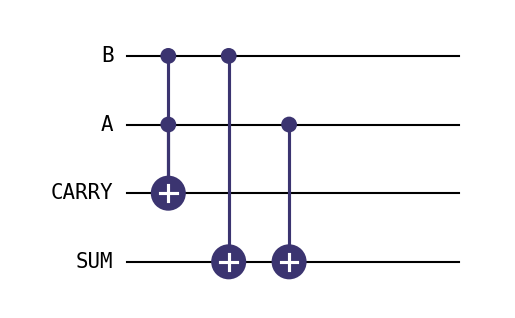
\includegraphics[width=0.5\textwidth]{problem3.png}
\end{center}

\bigskip
\begin{prob}
\end{prob}
\begin{enumerate}[label=(\alph*)]
    \item The oracle is defined as the operator which maps $\ket{s}$ to
        \[ O \ket{s} := \cos\theta \ket{s'} - \sin\theta \ket{q} \]
        and the diffuser is defined as the operator
        \[ D := 2 \ket{s}\bra{s} - I. \]
        We can rewrite $D$ as \begin{align*}
            D &= 2 \left( \cos\theta \ket{s'} + \sin\theta \ket{q} \right) \left( \cos\theta \bra{s'} + \sin\theta \bra{q} \right) - (\ket{s'}\bra{s'} + \ket{q}\bra{q}) \\
              &= 2 \cos^2\theta \ket{s'}\bra{s'}+2\cos\theta \sin\theta \ket{s'}\bra{q} + 2\cos\theta\sin\theta\ket{q}\bra{s'}+2\sin^2\theta\ket{q}\bra{q}-\ket{s'}\bra{s'}-\ket{q}\bra{q}.
        \end{align*}
        When we apply that operator to $O\ket{s}$, we get \begin{align*}
            DO\ket{s} &= 2\cos^3\theta\ket{s'}-2\cos\theta\sin^2\theta\ket{s'}+2\cos^2\theta\sin\theta\ket{q}-2\sin^3\theta\ket{q}-\cos\theta\ket{s'}+\sin\theta\ket{q} \\
                      &= \left( \cos^3\theta -3\cos\theta\sin^2\theta \right) \ket{s'} + \left( 3\cos^2\theta\sin\theta-\sin^3\theta \right) \ket{q} \\
                      &= \cos(3\theta) \ket{s'} + \sin(3\theta) \ket{q}.
        \end{align*}
        For that last step, I used the ``triple-angle identity", which I will derive here:
        \begin{align*}
            e^{3i\theta} = \left( \cos\theta + i \sin\theta \right)^3 &= \cos^3\theta +3i\cos^2\theta\sin\theta-3\cos\theta\sin^2\theta-i\sin^3\theta \\
            \cos(3\theta) = \Re(e^{3i\theta}) &= \cos^3\theta -3\cos\theta\sin^2\theta \\
            \sin(3\theta) = \Im(e^{3i\theta}) &= 3\cos^2\theta\sin\theta - \sin^3\theta.
        \end{align*}
    \item Before applying Grover's step, the qubit is in an equal superposition of 4 states, meaning the coefficient of $\ket{q}$ is $1/2$ and the coefficient of $\ket{s'}$ is $\sqrt{3}/2$. That means we can say $\theta = \pi/6$, so
        \[ DO\ket{s} = \cos(\pi/2)\ket{s'}+\sin(\pi/2)\ket{q} = \ket{q}, \]
        which means after one step of Grover's algorithm, the system has a 100\% chance of being in the solution state.
\end{enumerate}

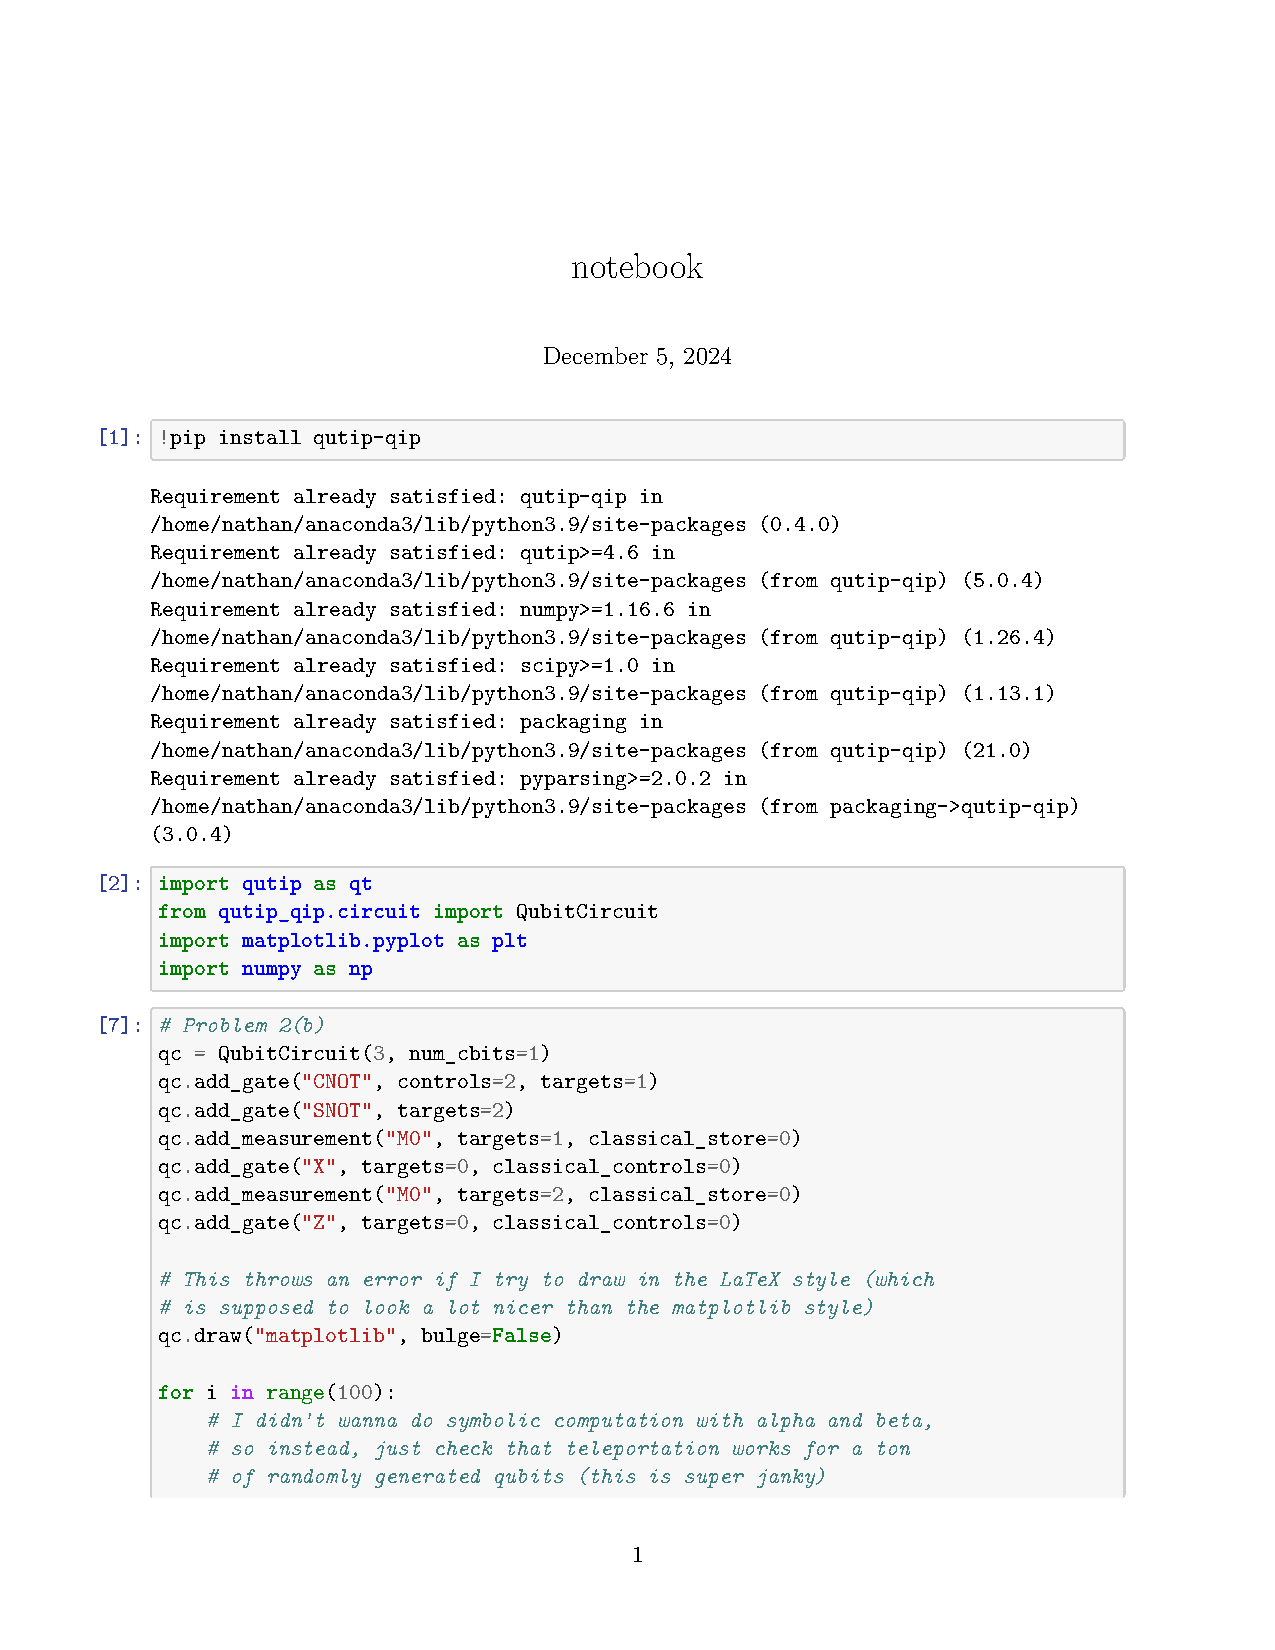
\includepdf[pages=-]{notebook.pdf}
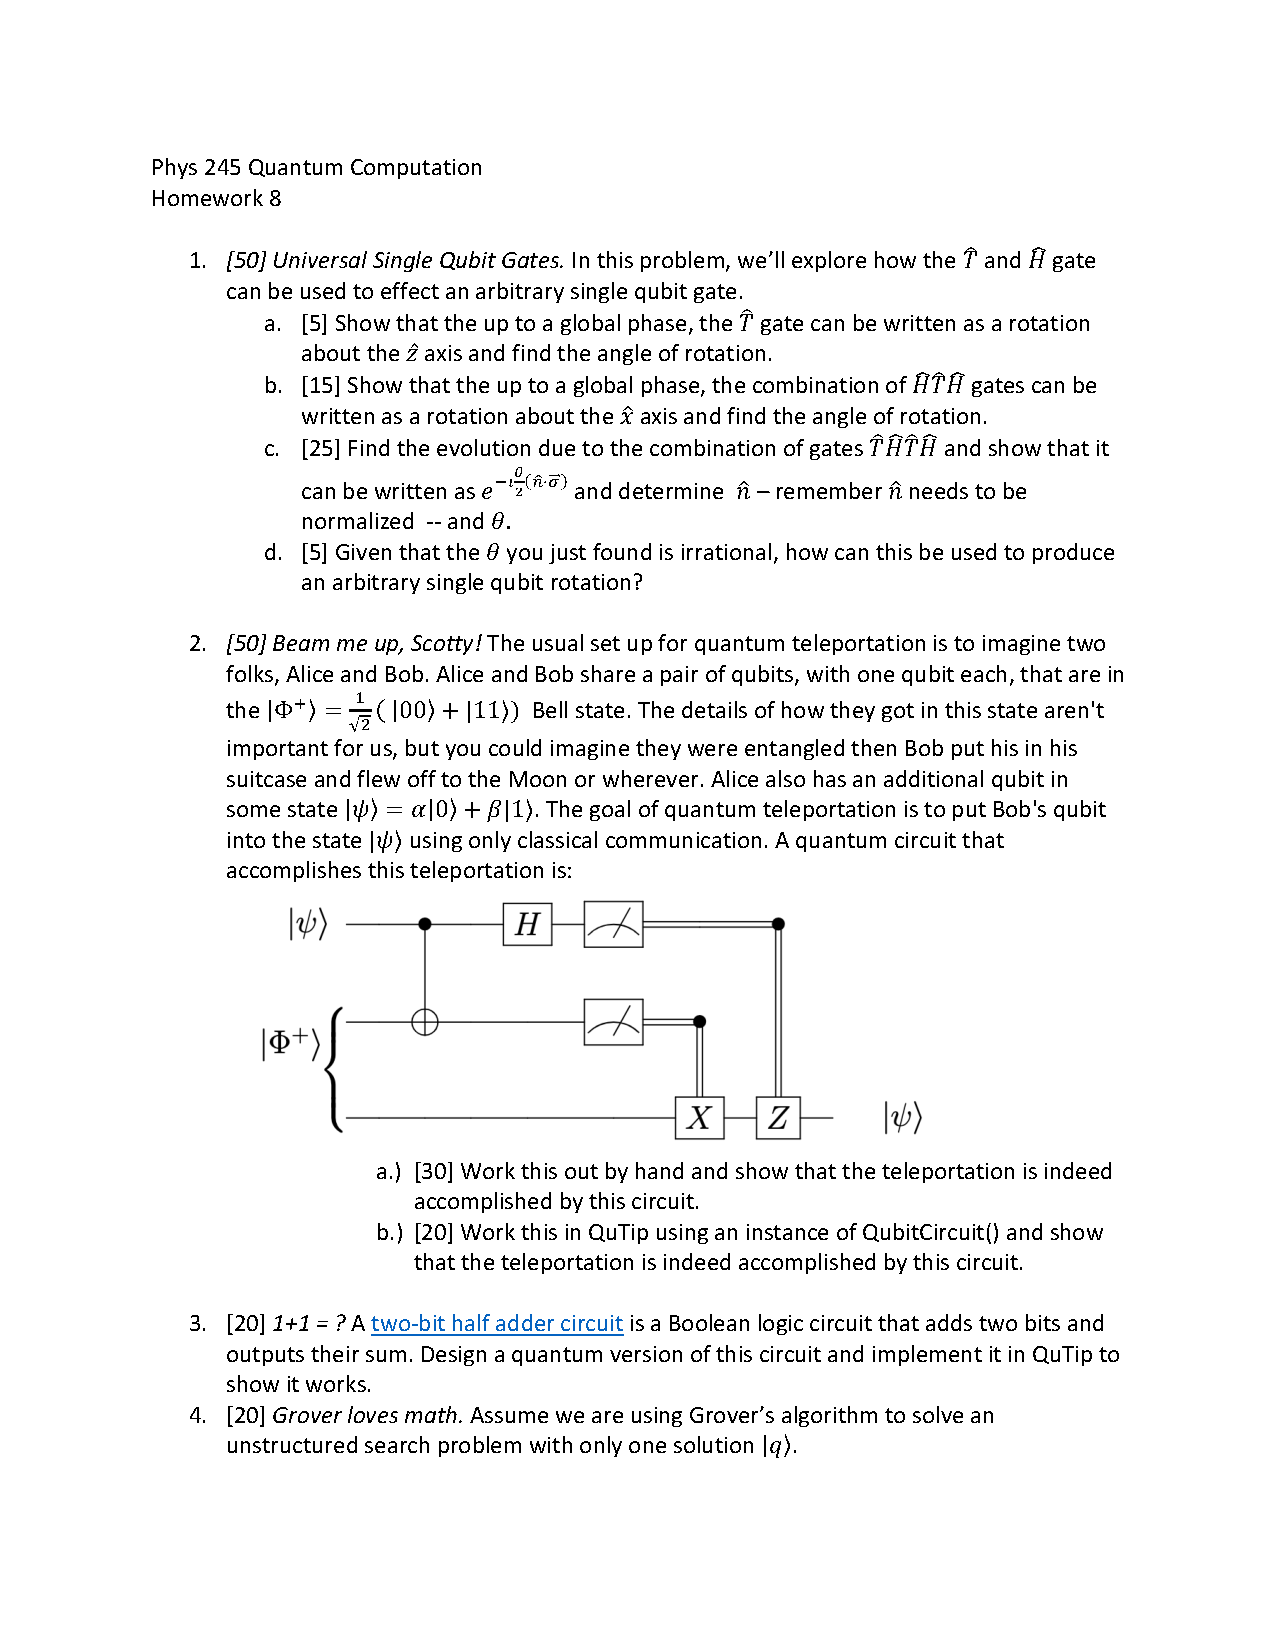
\includepdf[pages=-]{assignment.pdf}

\end{document}
